\documentclass[12pt]{article}
\usepackage{fullpage}
\usepackage[utf8]{inputenc}
\usepackage[T1]{fontenc}
\usepackage{microtype}
\usepackage{amssymb}
\usepackage{amsfonts}
\usepackage{float}
\usepackage{amsmath}
\usepackage{amsthm}
\usepackage{graphicx}
\usepackage[backend=bibtex,style=numeric]{biblatex}
\bibliography{citations}
\usepackage{wrapfig}
\usepackage{listings}
\usepackage{color}
\definecolor{dkgreen}{rgb}{0,0.6,0}
\definecolor{gray}{rgb}{0.5,0.5,0.5}
\definecolor{mauve}{rgb}{0.58,0,0.82}
\lstset{frame=tb,
  language=python,
  aboveskip=3mm,
  belowskip=3mm,
  showstringspaces=false,
  columns=flexible,
  basicstyle={\small\ttfamily},
  numbers=none,
  numberstyle=\tiny\color{gray},
  keywordstyle=\color{blue},
  commentstyle=\color{dkgreen},
  stringstyle=\color{mauve},
  breaklines=true,
  breakatwhitespace=true,
  tabsize=4
}
\graphicspath{{images/}}
\setlength{\parindent}{2em}
\setlength{\parskip}{0.25em}
\title{Instance Transfer with Boosting}
\author{David Blincoe}
\date{December 7, 2019}

\begin{document}
    \maketitle
    \section{Introduction} \label{boost-intro}
      One approach to inductive transfer learning is to use instances from the source and target
      domain to determine the overlap of the underlying data distributions. One approach to this
      is to define the {\it same-distribution} as the distribution under which the target domain falls,
      and the {\it diff-distribution} as the distribution under which the source domain falls. Again,
      one of the primary focuses of transfer learning is to avoid labeling target distribution examples.

      TrAdaBoost takes the approach of requiring some labeled target distribution data, or {\it same-distribution}
      data. The algorithms focus and goal is train on a large quantity of {\it diff-distribution} data that is
      supplemented with this small amount of {\it same-distribution} data. Logically, this can be thought of as
      an assumption that some of the {\it diff-distribution}’s data will fall within the {\it same-distribution}. A
      specific approach can be taken to transfer this underlying knowledge from the source to target goals.
      This is known as Instance-Transfer.

      One easy way to facilitate the learning of which examples from the {\it diff-distribution} is through
      weighting each example and allowing those examples weights to impact whether the learning. AdaBoost
      is very effective at iteratively weighting the training examples and determining which examples need
      to be considered more heavily than others.

      This works by increasing the weight of an example if the example was predicted incorrectly by the
      classifier. When an example is predicted correctly, it is assumed that the example is learned and
      the model has fit to it. The weight is then decreased and the algorithm assigns a weight to this
      iteration of the classifier. Once the algorithm either achieves an error of 0 or hits a maximum
      iteration cap, this process is suspended.

      Below, TrAdaBoost is presented along with a modification to allow for multiple sources of data

    \section{TrAdaBoost} \label{boost-tradaboost}
      TrAdaBoost operates in the same fashion except is updates the weights of the same-distribution and
      diff-distribution differently.

      \subsection{Formal Definition} \label{boost-tradaboost-def}
        Before describing the innerworkings of the algorithm some formal definitions must be defined.

        Let there be some sample space $X_S$ that falls under the {\it same-distribution} and another sample space $X_D$
        that is under the {\it diff-distribution}. The label sample space is defined as $Y= \{0,1\}$. Together, $X_S \bigcup X_D = X$
        defined the entire sample space under which TrAdaBoost will operate.

        The train data for the algorithm is defined as two sets, $T_D$ and $T_S$. $T_D = \{(x^d_i, f(x^d_i)\}$ where $x^d_i \in X_D$ and
        $(i = 1, \dots, m)$. $T_S = \{(x^s_i, f(x^s_i)\}$ where $x^s_i \in X_S$ and $(i = 1, \dots, n)$. Here $m$ and $n$ are the sizes of
        two sets. Here $f(x)$ defines the function mapping the example from the given sample space to the output space. Together these sets
        form the training data. \autocite{dai_yang_xue_yu_2007}

        \begin{equation}
          x_i =
          \begin{cases}
            x_i^d        & i = 1, \dots, m \\
            x_i^s        & i = m + 1, \dots, n+m
          \end{cases}
        \end{equation}

        The testing data is defined as one set, $S$. $S = \{(x_i^t)\}$ where $x_i^t \in X_S$ and $(i=1, \dots, k)$. $K$ is the size of 
        the test set. \autocite{dai_yang_xue_yu_2007}

        Logically, the above definitions are as follow. $T_D$ is the data from the {\it diff-distribution} that is being reused to learn 
        this problem and $T_S$ is from the limited amount of labeled data in {\it same-distribution}. The overall goal of our classifier is
        to learn some function $\hat{f}$ such that the training and testing error is minimized.

      \subsection{Algorithm} \label{boost-tradaboost-algo}

        This modification to AdaBoost follows the same procedure as in normal AdaBoost, except for the weighting of the $T_D$ data. As in
        AdaBoost, when an example from the $T_S$ set is predicted correctly, it is assumed learned and its weight is decreased and when it
        is predicted incorrectly, the examples weight is increased. For the $T_D$ data, when the model predicts an example incorrectly,
        an assumption is made that this example lies outside of the {\it same-distribution} and the example weight is decreased. Likewise,
        the inverse applies.

        \begin{figure}[H]
          \centering
          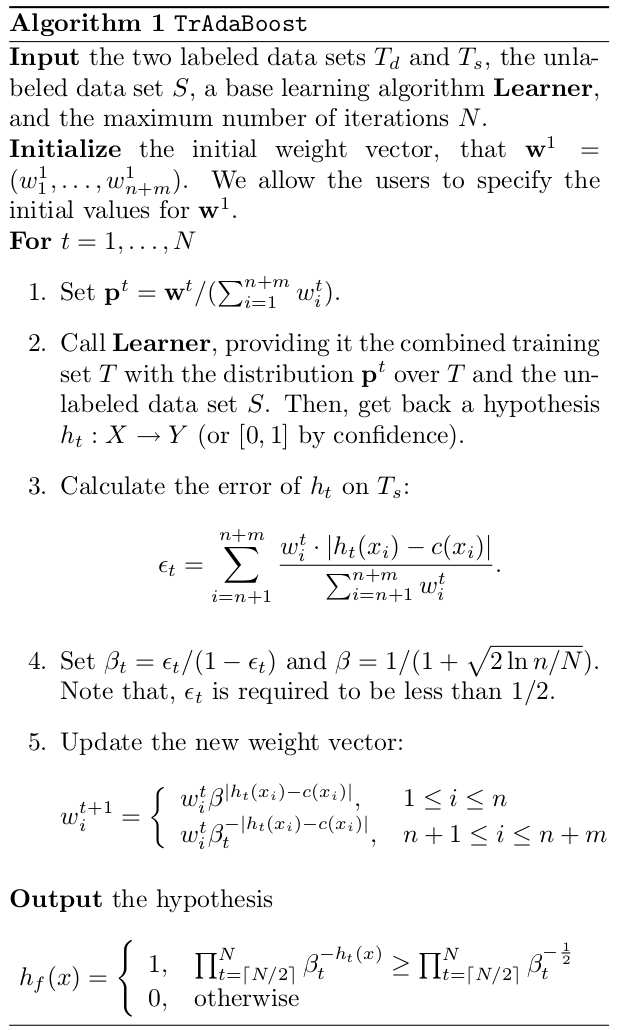
\includegraphics[width=0.6\textwidth]{tradaboost-algorithm.png}
          \caption{TrAdaBoost Algorithm \autocite{dai_yang_xue_yu_2007}}
          \label{tradaboost-algorithm}
        \end{figure}

      \subsection{Theory} \label{boost-tradaboost-theory}



    \section{Mutlisource TrAdaBoost} \label{boost-multisource}

      \subsection{Formal Definition} \label{boost-multi-def}

      \subsection{Algorithm} \label{boost-multi-algo}

      \subsection{Theory} \label{boost-multi-theory}

      \subsection{Weighting Multisource TrAdaBoost} \label{boost-multisource-weight}
      
    \printbibliography
\end{document}